%CAPITULO VI , Análisis de resultados

%Una cosa es lo que se propuso resolver y otra lo que realmente se obtuvo, en esta etapa se analizan los resultados obtenidos como parte del desarrollo del trabajo de investigación. 

\chapter{ ANÁLISIS DE RESULTADOS }

\textit{Es necesario reportar de manera final cual es prototipo y los resultados que se obtuvieron, esto con el fin de generar las conclusiones utilizando los resultados del prototipo generado.}

\section{ Prueba No. 1 - Sistema eléctrico de 4 fases (Calibración)}

La figura \ref{Graficas} contiene la medición de 3 fases utilizando el sistema de medición conectado para realizar una medición no invasiva en un sistema lineal, con una carga netamente resistiva

\subsection{ Objetivo de la prueba}

Verificar el adecuado funcionamiento del dispositivo electrónico, calibrar el software contra dispositivos certificados de nombre reconocido para obtener una medición lo mas exacta posible, con la finalidad de realizar mediciones con la mayor certidumbre posible \cite{NOM}.

\subsection{ Procedimiento}

En el neutro el sensor de corriente correspondiente al puerto CT1 del circuito implementado, por ley de nodos, al ser la carga bajo medición un circuito en con una resistencia en serie, la corriente que fluye por toda la maya debe ser igual en la fase y el neutro, por lo que se procede a realizar la medición.

\begin{figure}[H]
	\begin{center}
 		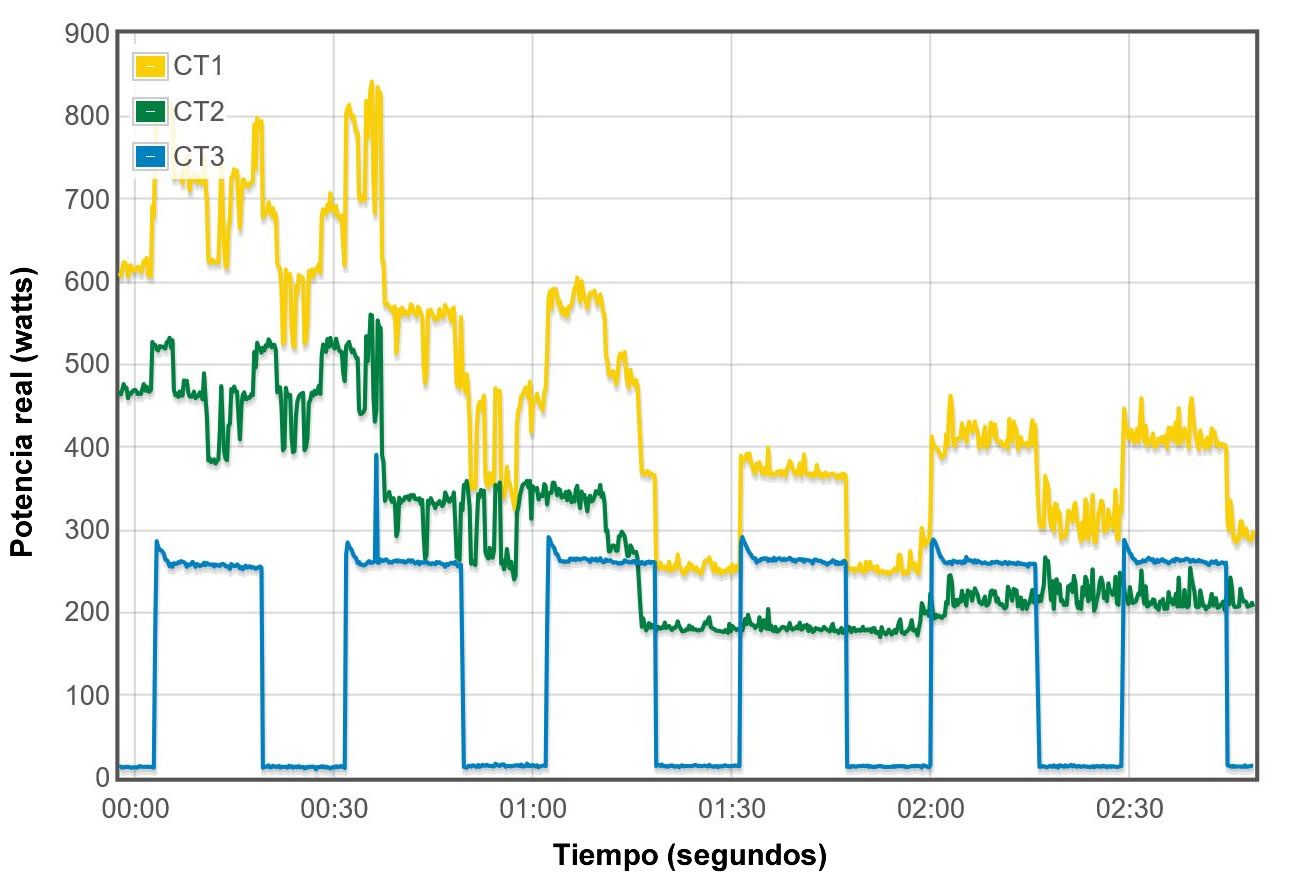
\includegraphics[width = .85\textwidth]{Tesis/Imagenes/Grafica.JPG}
 		\captionof{figure}{Gráfica en tiempo del sistema de medición} 
	\label{Graficas}
    \end{center} 
\end{figure}



